\documentclass{WileyMSP-template}

\begin{document}


\pagestyle{fancy}
\rhead{\includegraphics[width=2.5cm]{vch-logo.png}}


\title{Influence of illumination spectrum on dissociation kinetic of iron-boron pairs in silicon}

\maketitle



% Author: Please give full first and last names for authors and include * after the name of all corresponding authors

\author{Oleg Olikh*}
\author{Oleksandr Datsenko}
\author{Serhiy Kondratenko}

% Dedication

\dedication{}






% Affiliations: Please provide adacemic titles (Prof. or Dr.) for all authors where applicable, and include an institutional email address for all corresponding authors
\begin{affiliations}
Prof. O. Olikh, Dr. O. Datsenko, Prof. S. Kondratenko\\
Taras Shevchenko National University of Kyiv, 64/13, Volodymyrska Street, 01601, Kyiv, Ukraine\\
Email Address: olegolikh@knu.ua

%A. N. O. Author\\
%Address

\end{affiliations}


% Keywords: Please provide a minimum of three and a maximum of seven keywords, separated by commas

\keywords{silicon, iron-boron pairs, light-induced dissociation}



% Abstract should be written in the present tense and impersonal style (i.e., avoid we), and be at most 200 words long
\begin{abstract}

Please insert your abstract here

\end{abstract}

% Text: Please use section headings and subheadings as specified below. For communications, all section headings apart from Experimental Section should be removed
% Please make the first reference to a display item bold: \textbf{Figure 1}
% Do not abbreviate Figure, Equation, etc.; display items are always singular, i.e., Figure 1 and 2.
% Equations are always singular, i.e., Equation 1 and 2, and should be inserted using the {equation} environment, not as graphics
% Please do not use footnotes in the text, additional information can be added to the Reference list.


\section{Introduction}

Defects significantly impact semiconductor properties.
Although minimizing device dimensions to nanometers shifts some focus from extensive to point defects,
physical properties still rely heavily on the presence and distribution of these irregularities.
Hence, many strategies for enhancing semiconductor structures, including radiation and temperature treatments or certain fabrication conditions, strive to decrease the defect concentration or neutralize its effects \cite{Cai2023,Vobecky2021,Frascaroli2021}.
For instance, in the case of photovoltaic devices, we must understand and optimize the carrier properties tied to defects and impurities  \cite{Cai2023}.
Such controlled alteration methods of the defective subsystem have been generalized under the term ``defect engineering'' and are extremely important from a practical standpoint.

Successful defect engineering hinges on an in-depth understanding of defect properties.
Key factors are defect formation energy, transition energy levels, self-compensating effects, nonradiative recombination caused by defects,
and the mechanism of reconstruction and diffusion  \cite{Cai2023}.
Considering the extraordinary diversity of possible intrinsic and impurity defects, complete information on all of them is lacking even for silicon, which is the most studied semiconductor.
Nevertheless, it must be noted that considerable data have been amassed on silicon, and have a solid understanding of some defects \cite{Juhl2018}.

For instance, such defects are iron impurity, a common, detrimental, and often unavoidable contaminant
in photovoltaic silicon \cite{Frascaroli2021,Sun2021}, and iron-boron pair.
Specifically, iron atoms are known to be at the interstitial sites, and Fe$_i^+$ are highly efficient recombination centers \cite{WeberFe}.
In p-type Si at room temperature, iron atoms are almost predominantly bound in complexes with dopants (B, Ga, Al, In).
This defect demonstrates bistable behavior: the stable state is defined by the configuration in which the Fe occupies
the first nearest tetrahedral interstitial site closest to the substituent atom,
whereas, in the metastable configuration, Fe is at the second $T_d$ interstitial site \cite{FeB:PhysRevB49}.
The energy levels associated with iron and its complexes, as well as the respective carriers capture cross-sections, are well-established \cite{Juhl2018,ROUGIEUX2018}.
Among the acceptor-iron pairs, the complex FeB is the most thoroughly investigated,
primarily due to the widespread use of Si:B in the fabrication of various devices, such as solar cells.
However, it is worth mentioning that gallium is gaining increasing attention as an acceptor dopant whose incorporation,
for instance, can help mitigate the light and elevated temperature-induced degradation \cite{Ning2022}.

It is known that
FeB pairs can be dissociated by illumination, minority carrier injection and thermal treatment at 200~$^\circ$ \cite{FeBAssJAP2014}.





\begin{figure}
\centering
  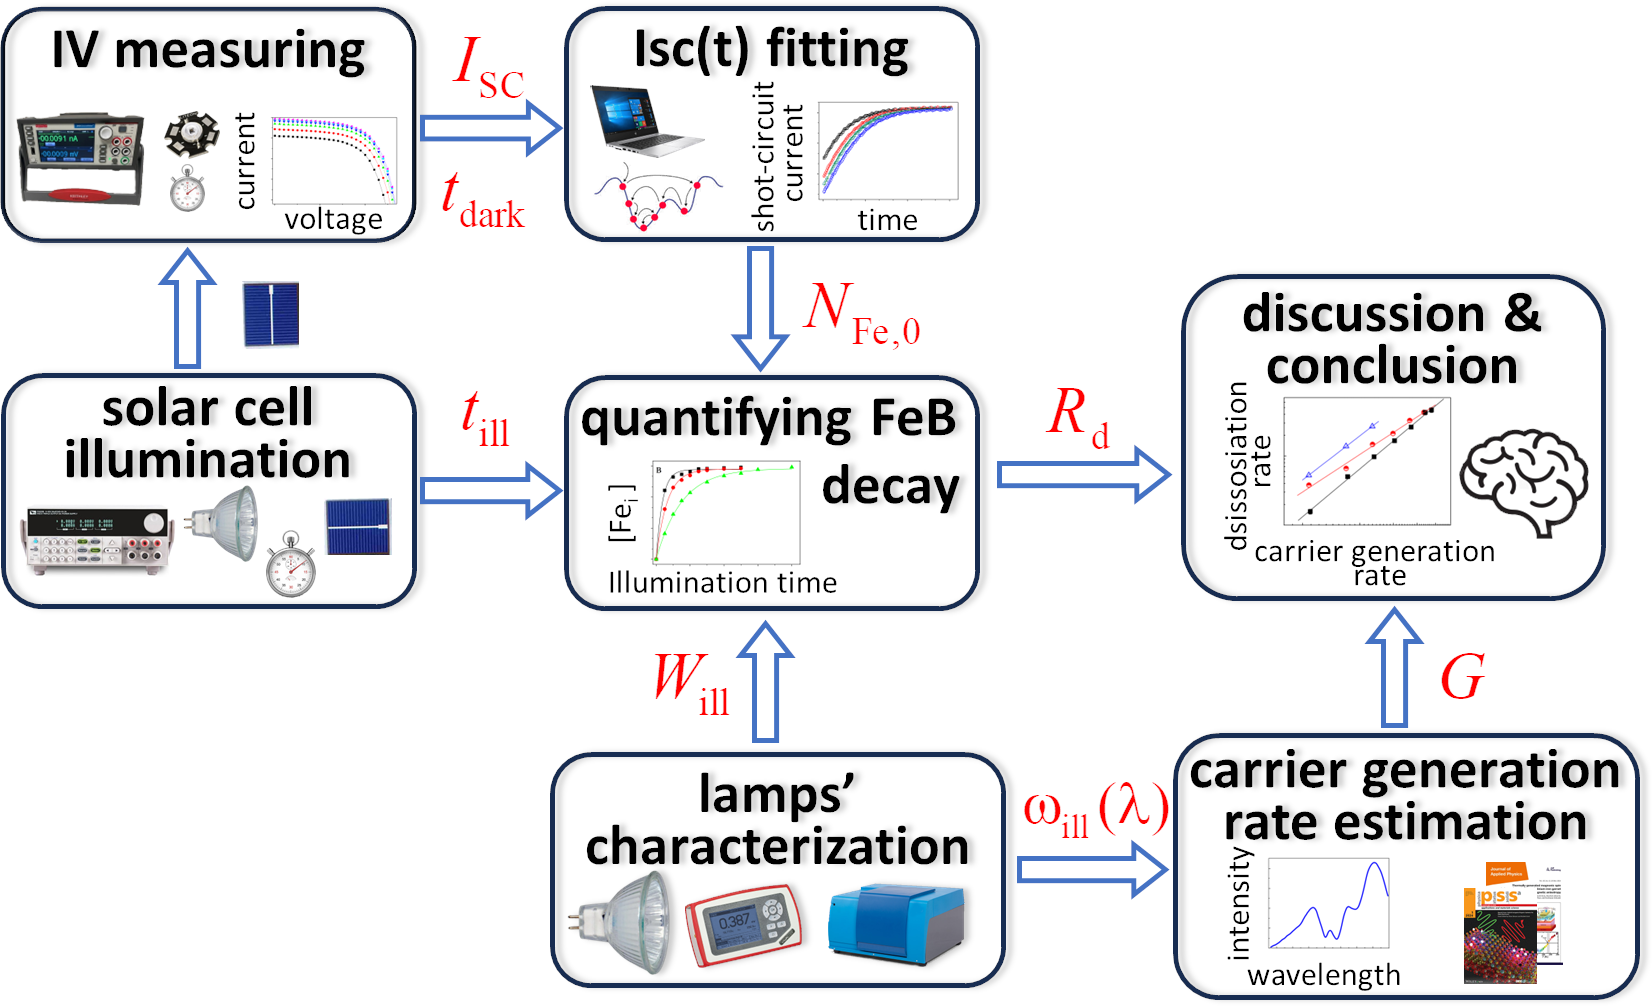
\includegraphics[width=0.5\linewidth]{Fig1.png}
  \caption{Investigation framework}
  \label{fig1}
\end{figure}


%\subsection{First Subsection}
%
%
%\subsubsection{First Sub Subsection}
%
%
%\threesubsection{First lowest-level subsection}


\section{Results and Discussion}
\subsection{First Subsection}

\begin{figure}
\centering
  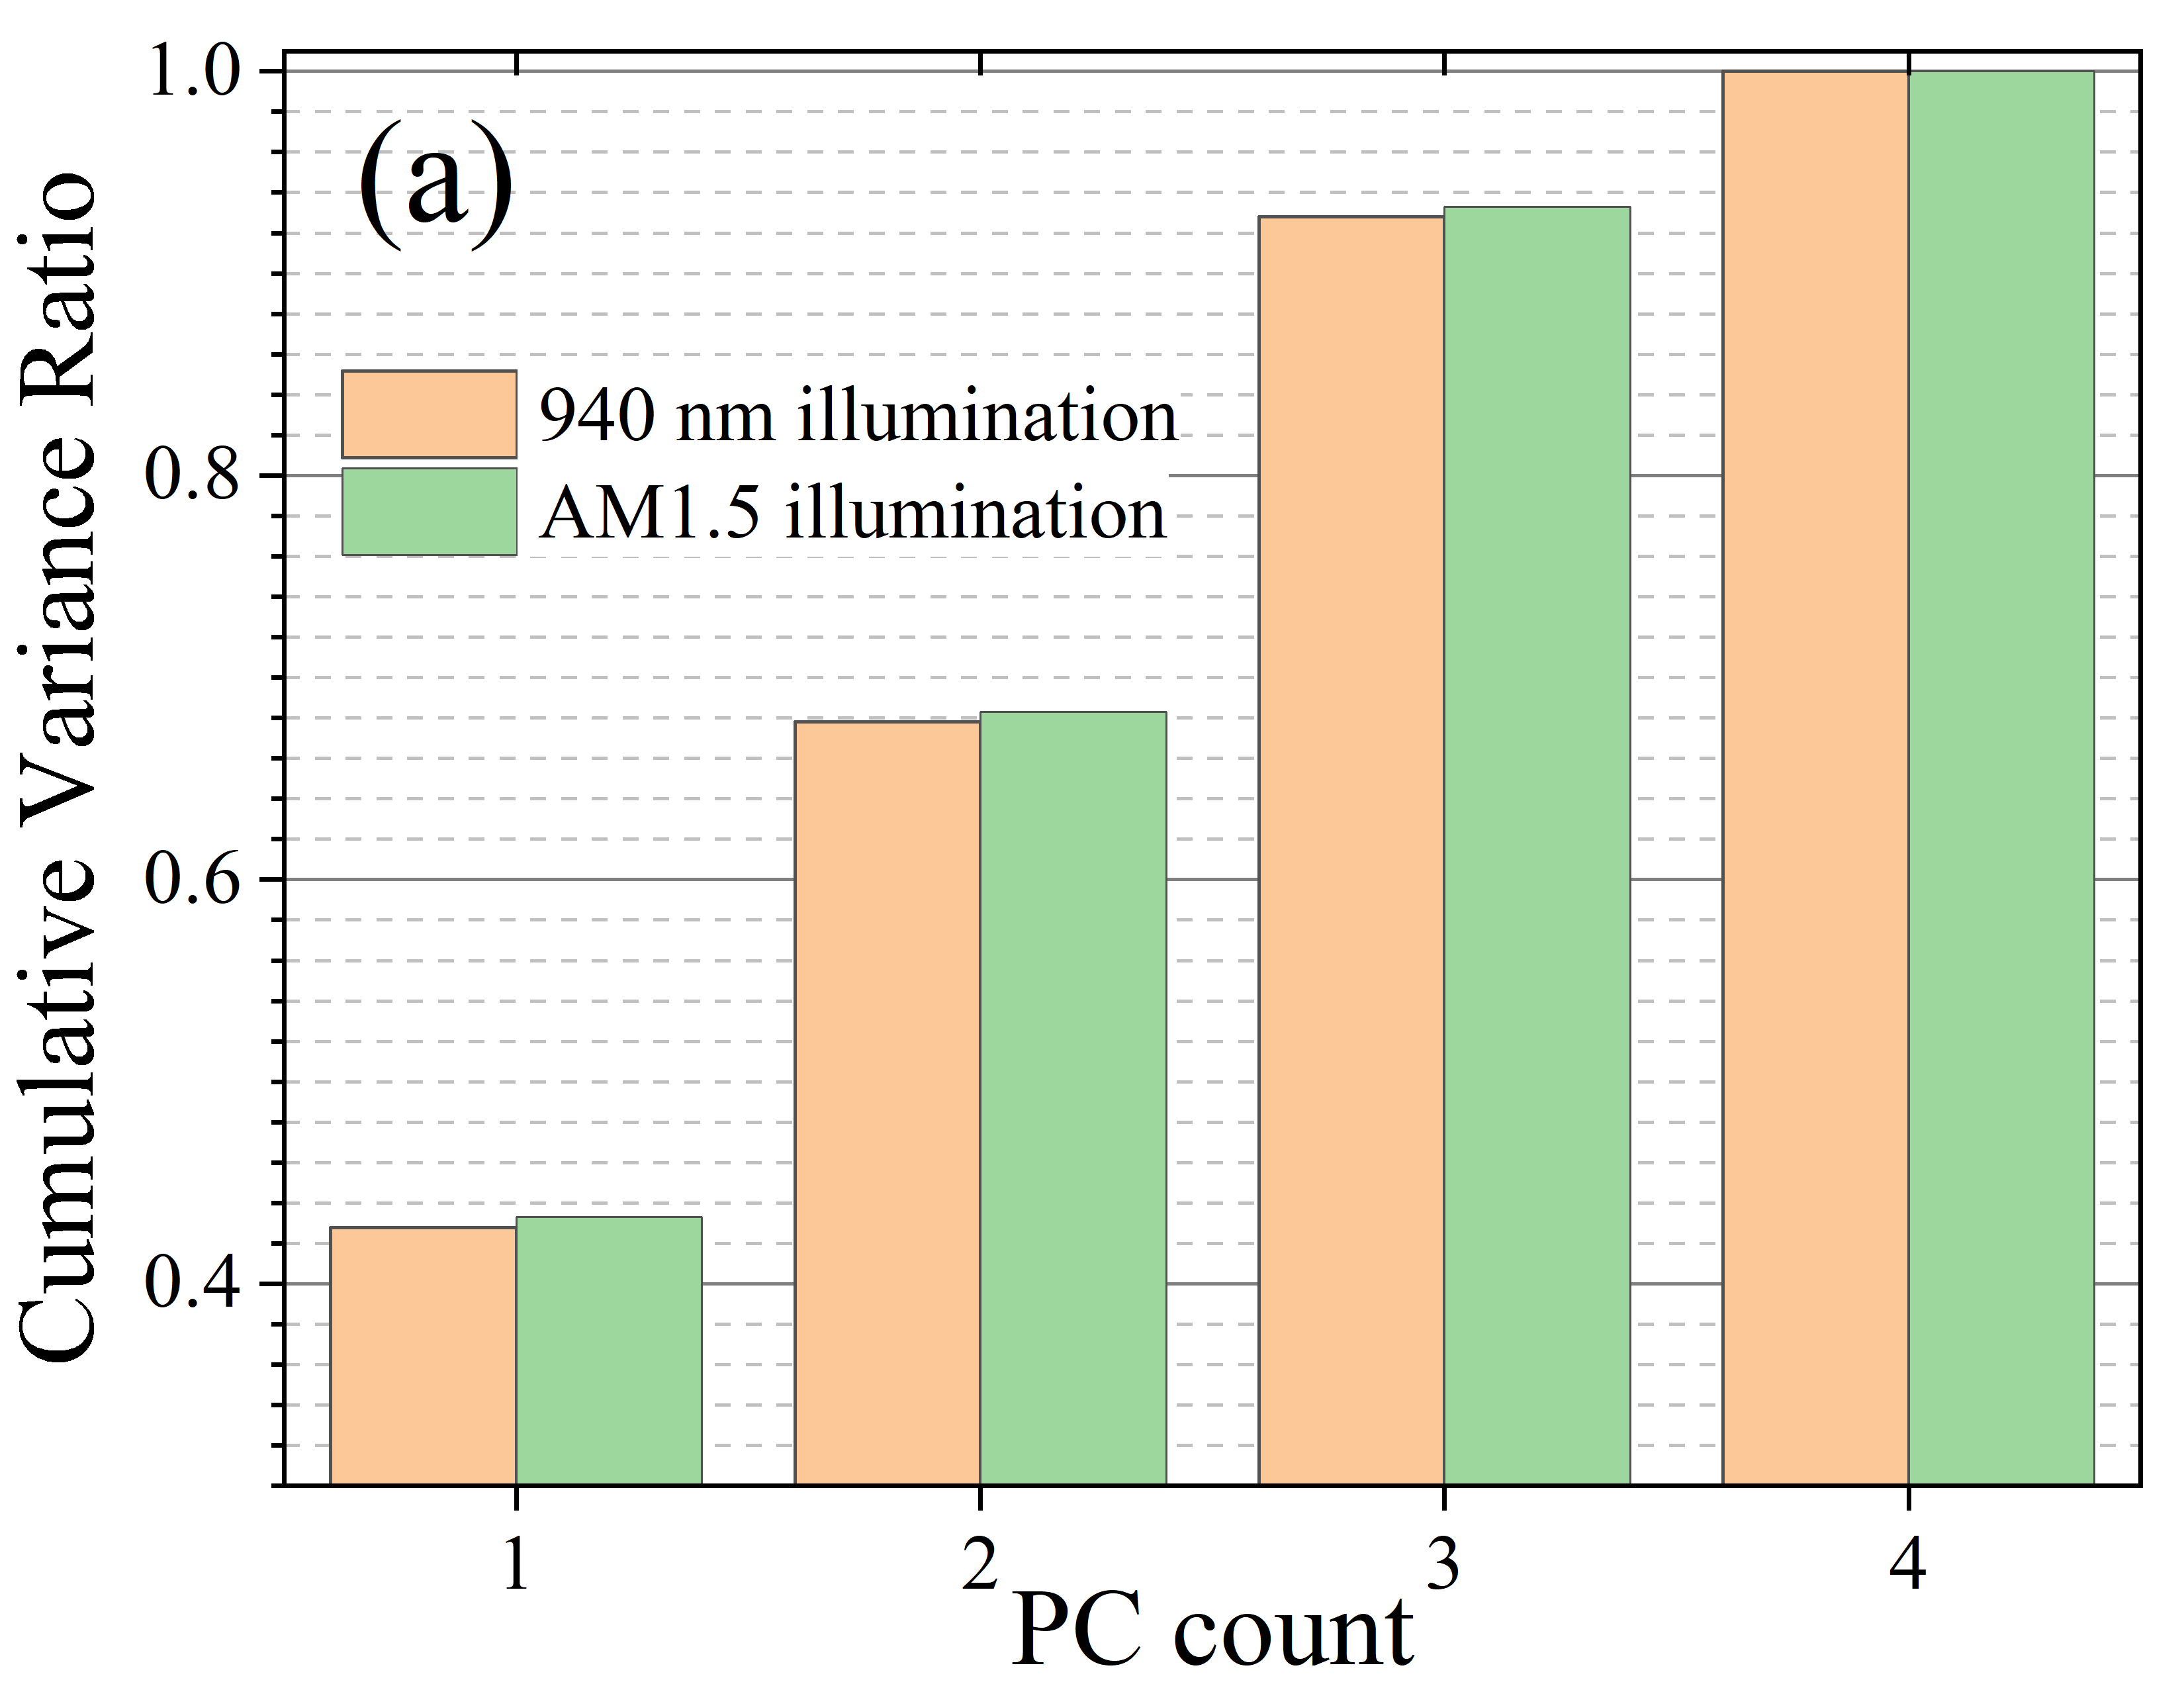
\includegraphics[width=0.4\linewidth]{Fig2a.png}
  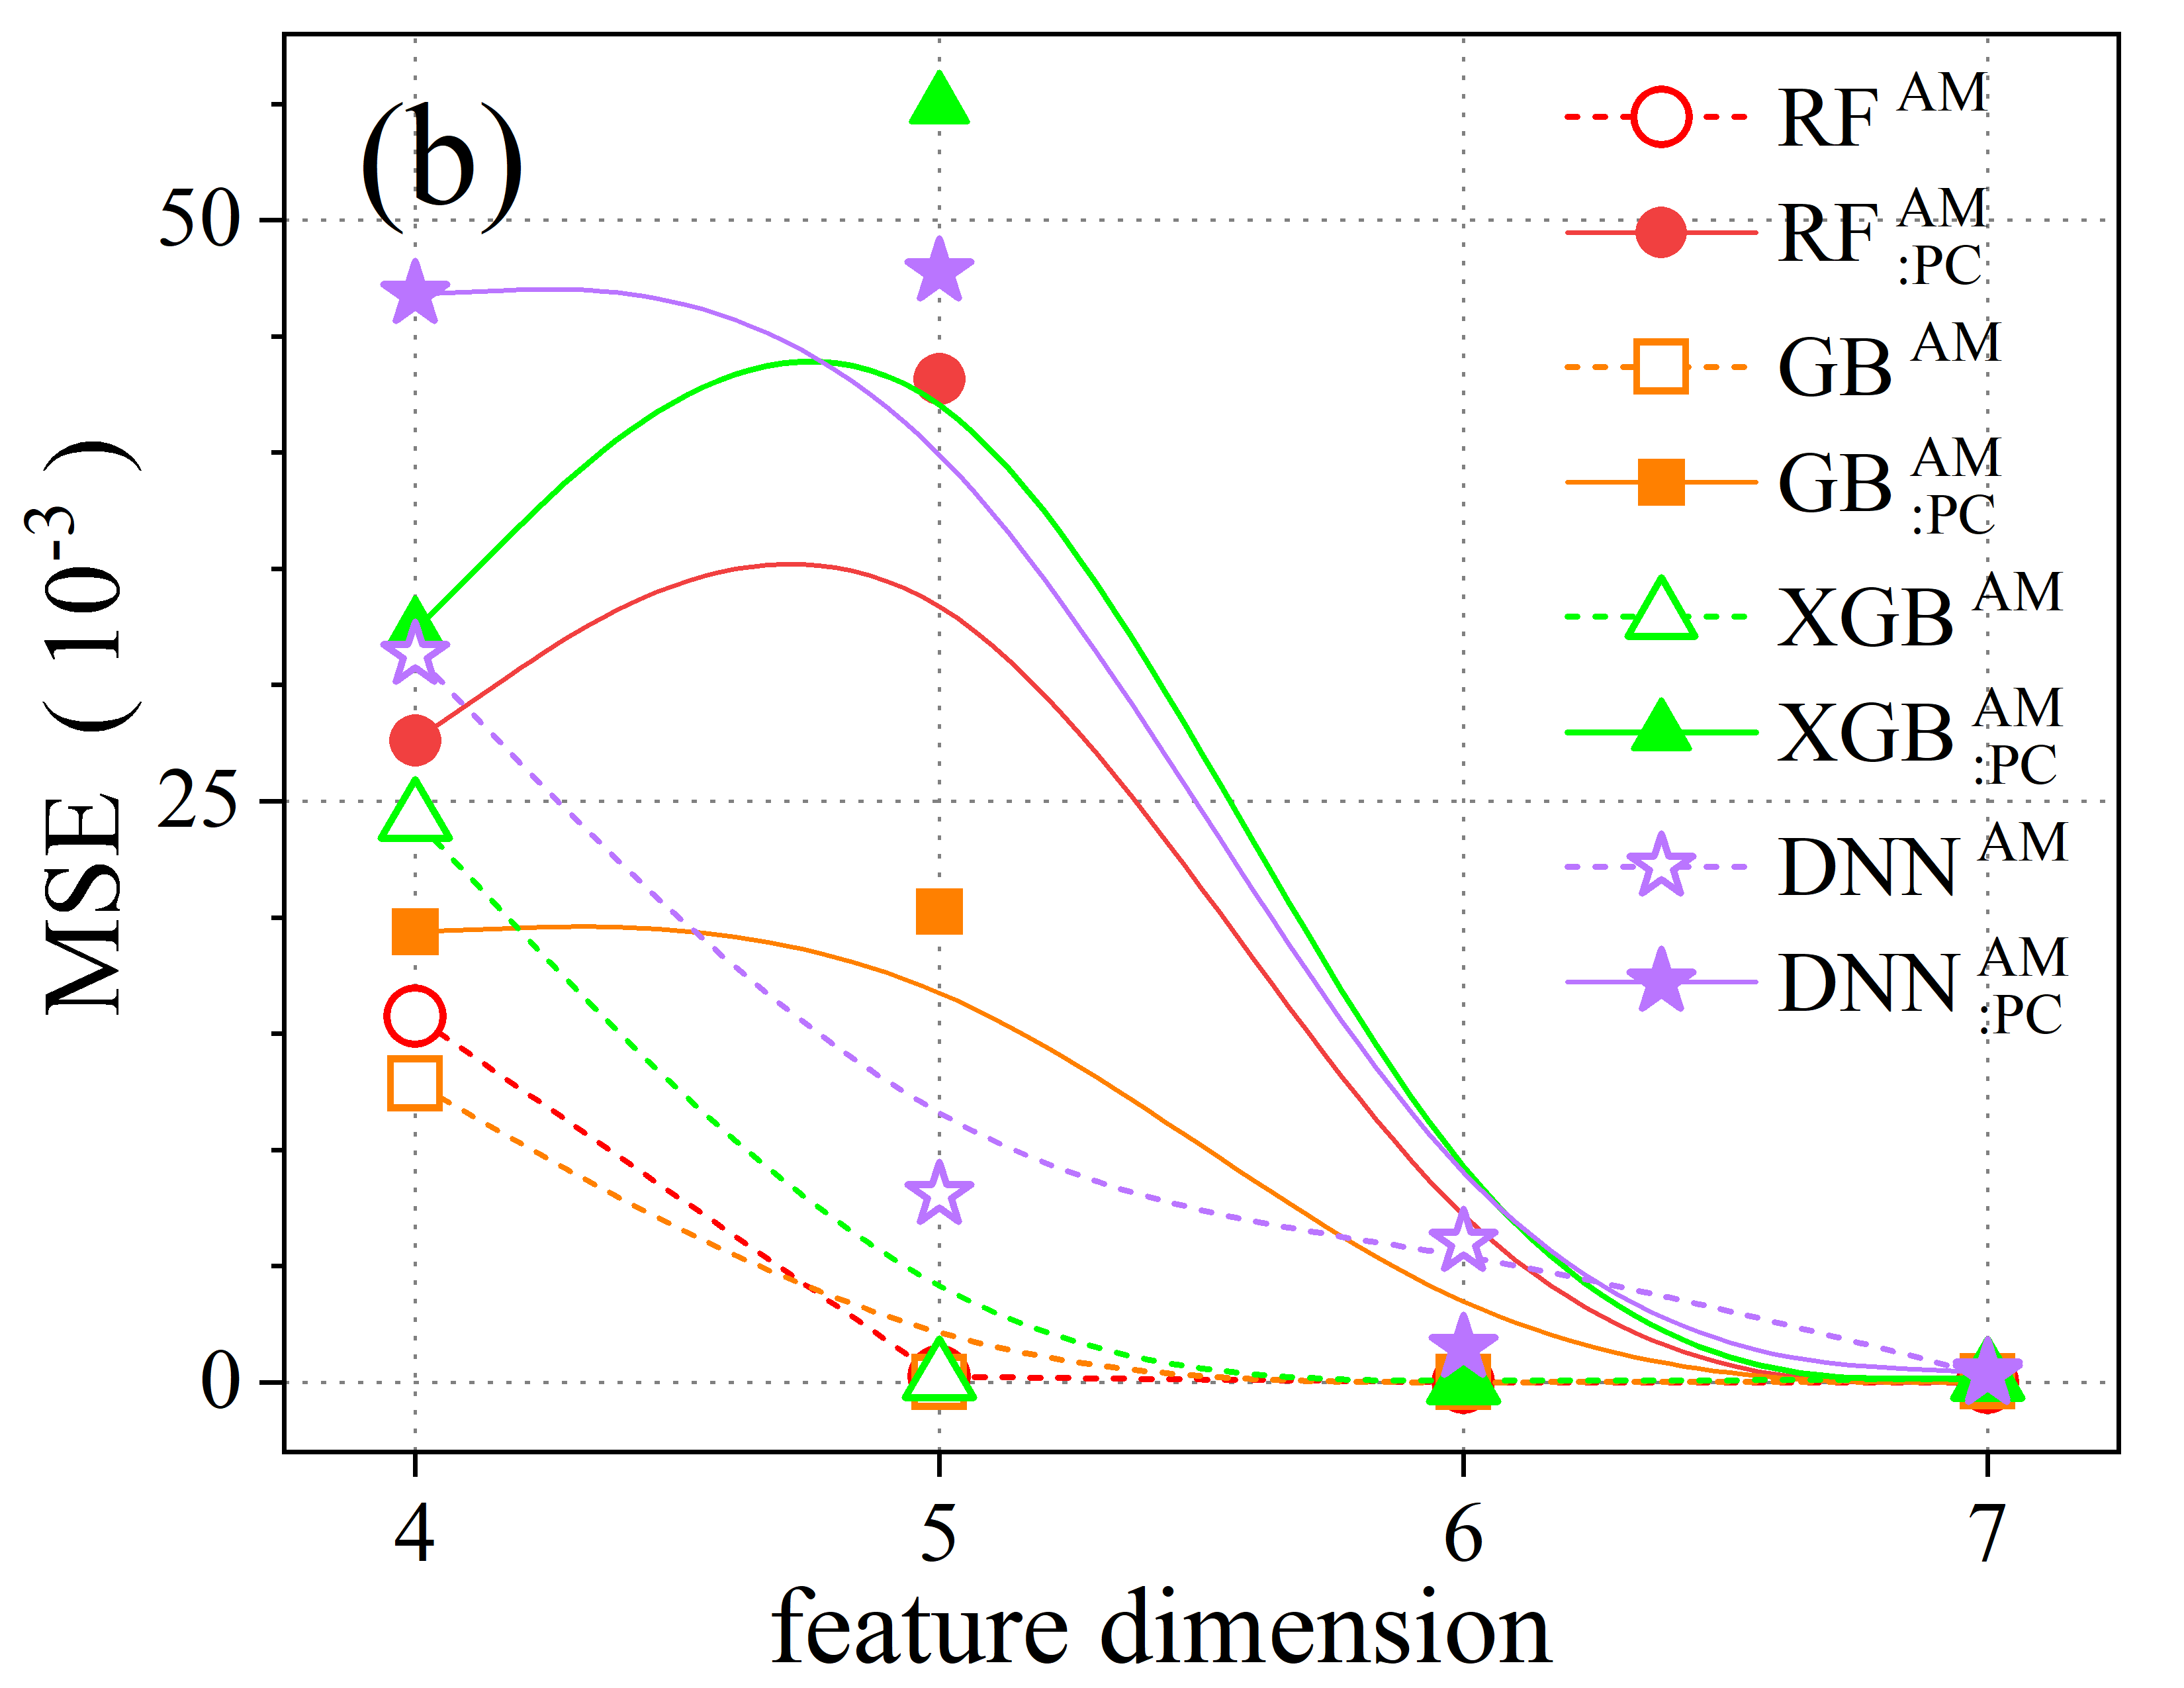
\includegraphics[width=0.4\linewidth]{Fig2b.png}
  \caption{Typical current-voltage characteristics measured 
  under low-intensive (LED) illumination across different periods following exposure to strong light (halogen lamp) (panel a) and 
  short circuit current plotted as a function of the time after high-intensive illumination (panel b).
  %The marks are the experimental results and the lines are given for convenience only (b) and the curves fitted according to \cite{Olikh2022:JMatSci,Olikh2021JAP}.
  The marks are the experimental results and the lines on panel b are the curves fitted according to \cite{Olikh2022:JMatSci,Olikh2021JAP}.
  Light sources: GE (a), Osram (b).
  $t_\mathrm{ill}$, s: 50 (a), 5(b). 
  $W_\mathrm{ill}=50$~mW (b).
  $T=340$~K.}
  \label{fig2}
\end{figure}

\begin{figure}
\centering
  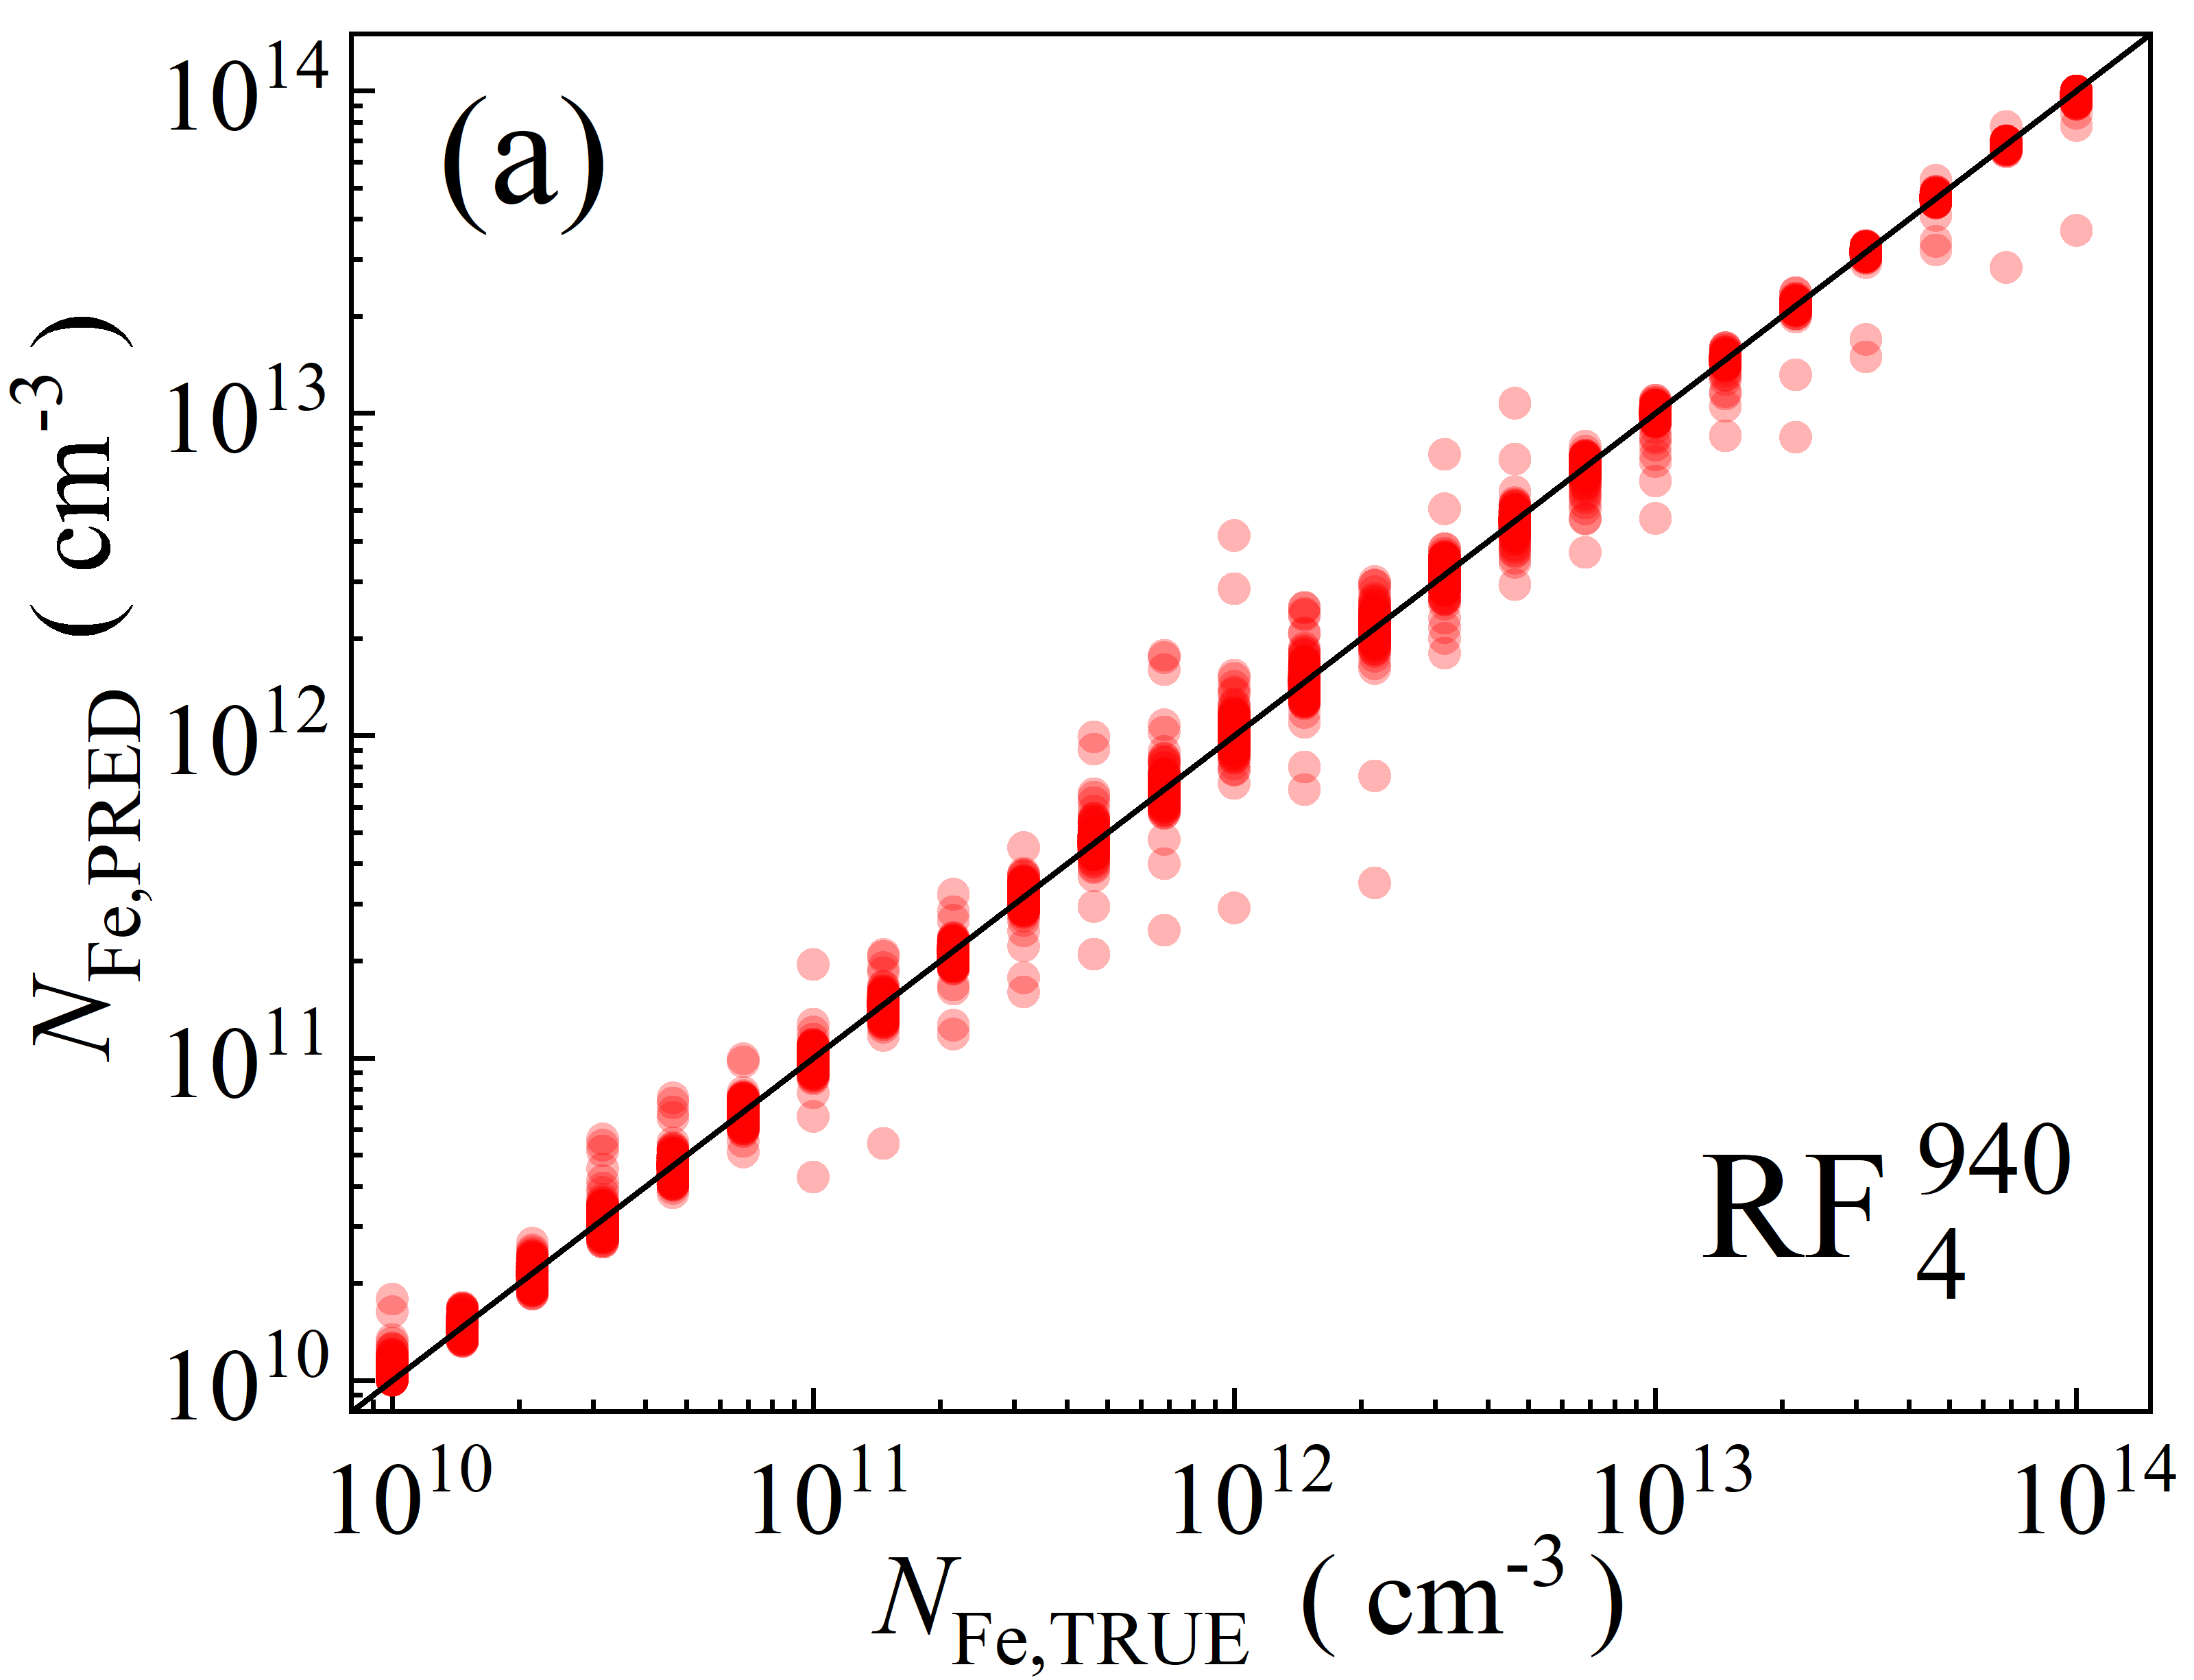
\includegraphics[width=0.4\linewidth]{Fig3a.png}
  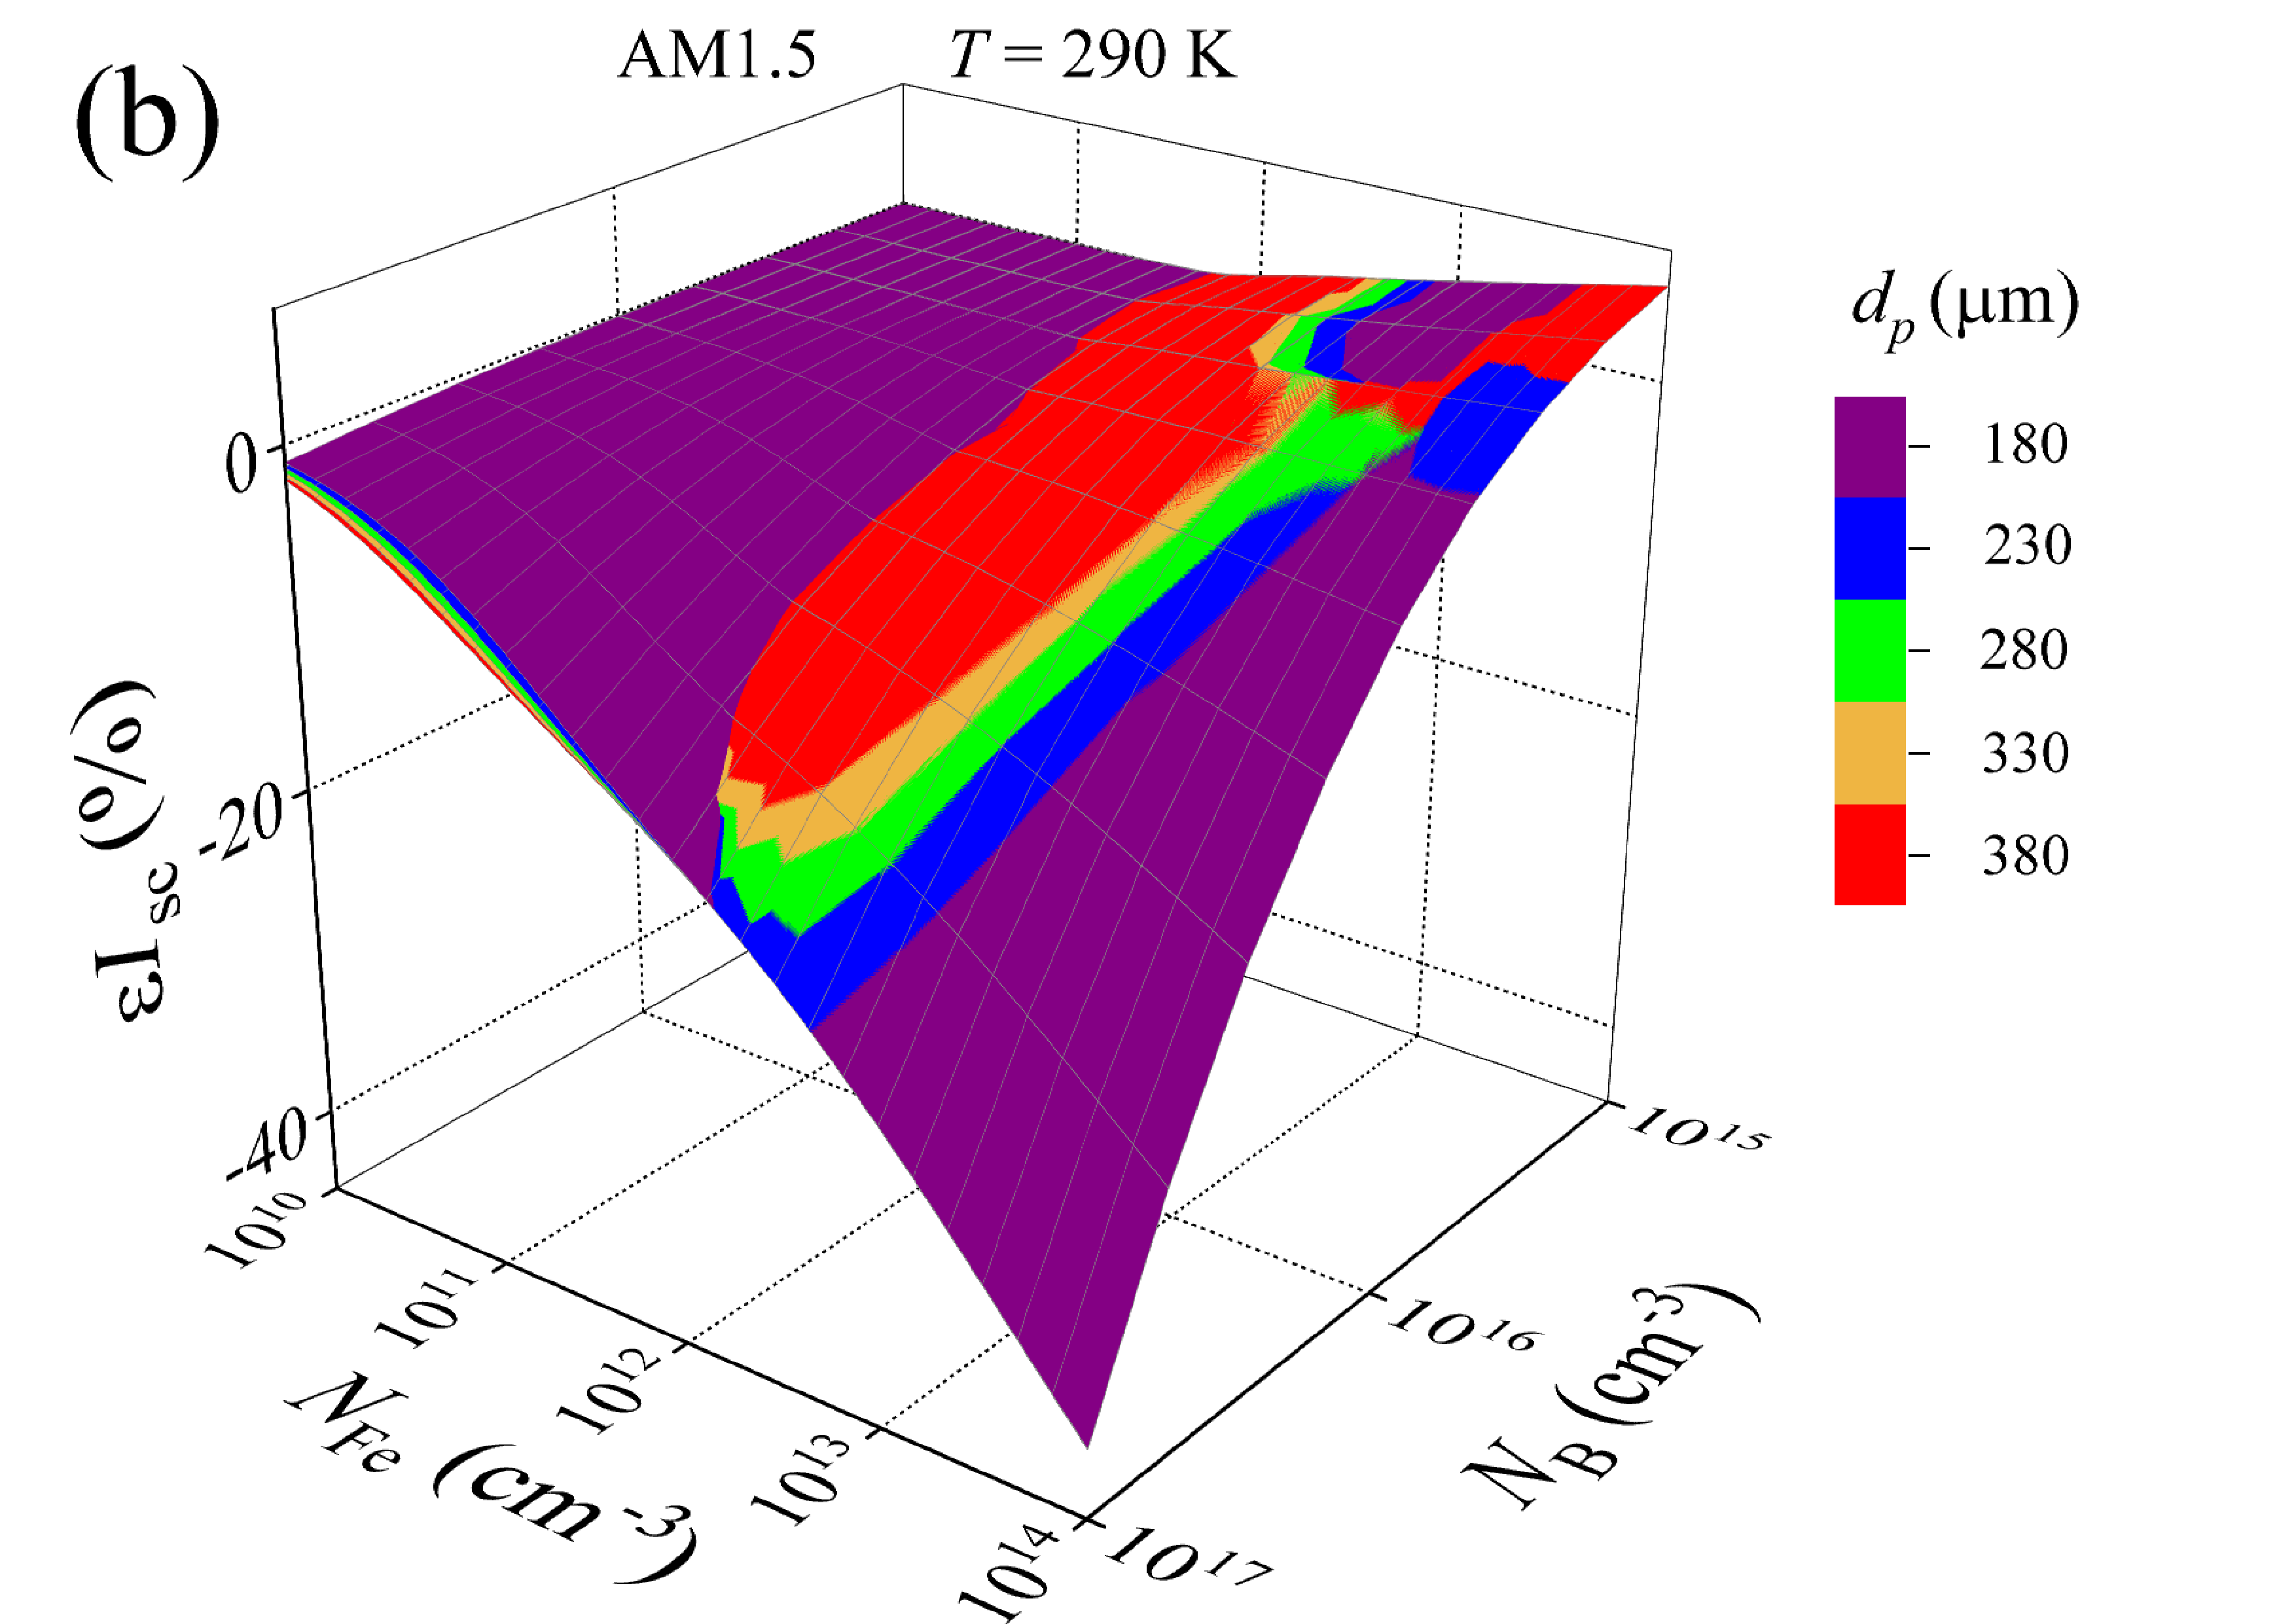
\includegraphics[width=0.4\linewidth]{Fig3b.png}
  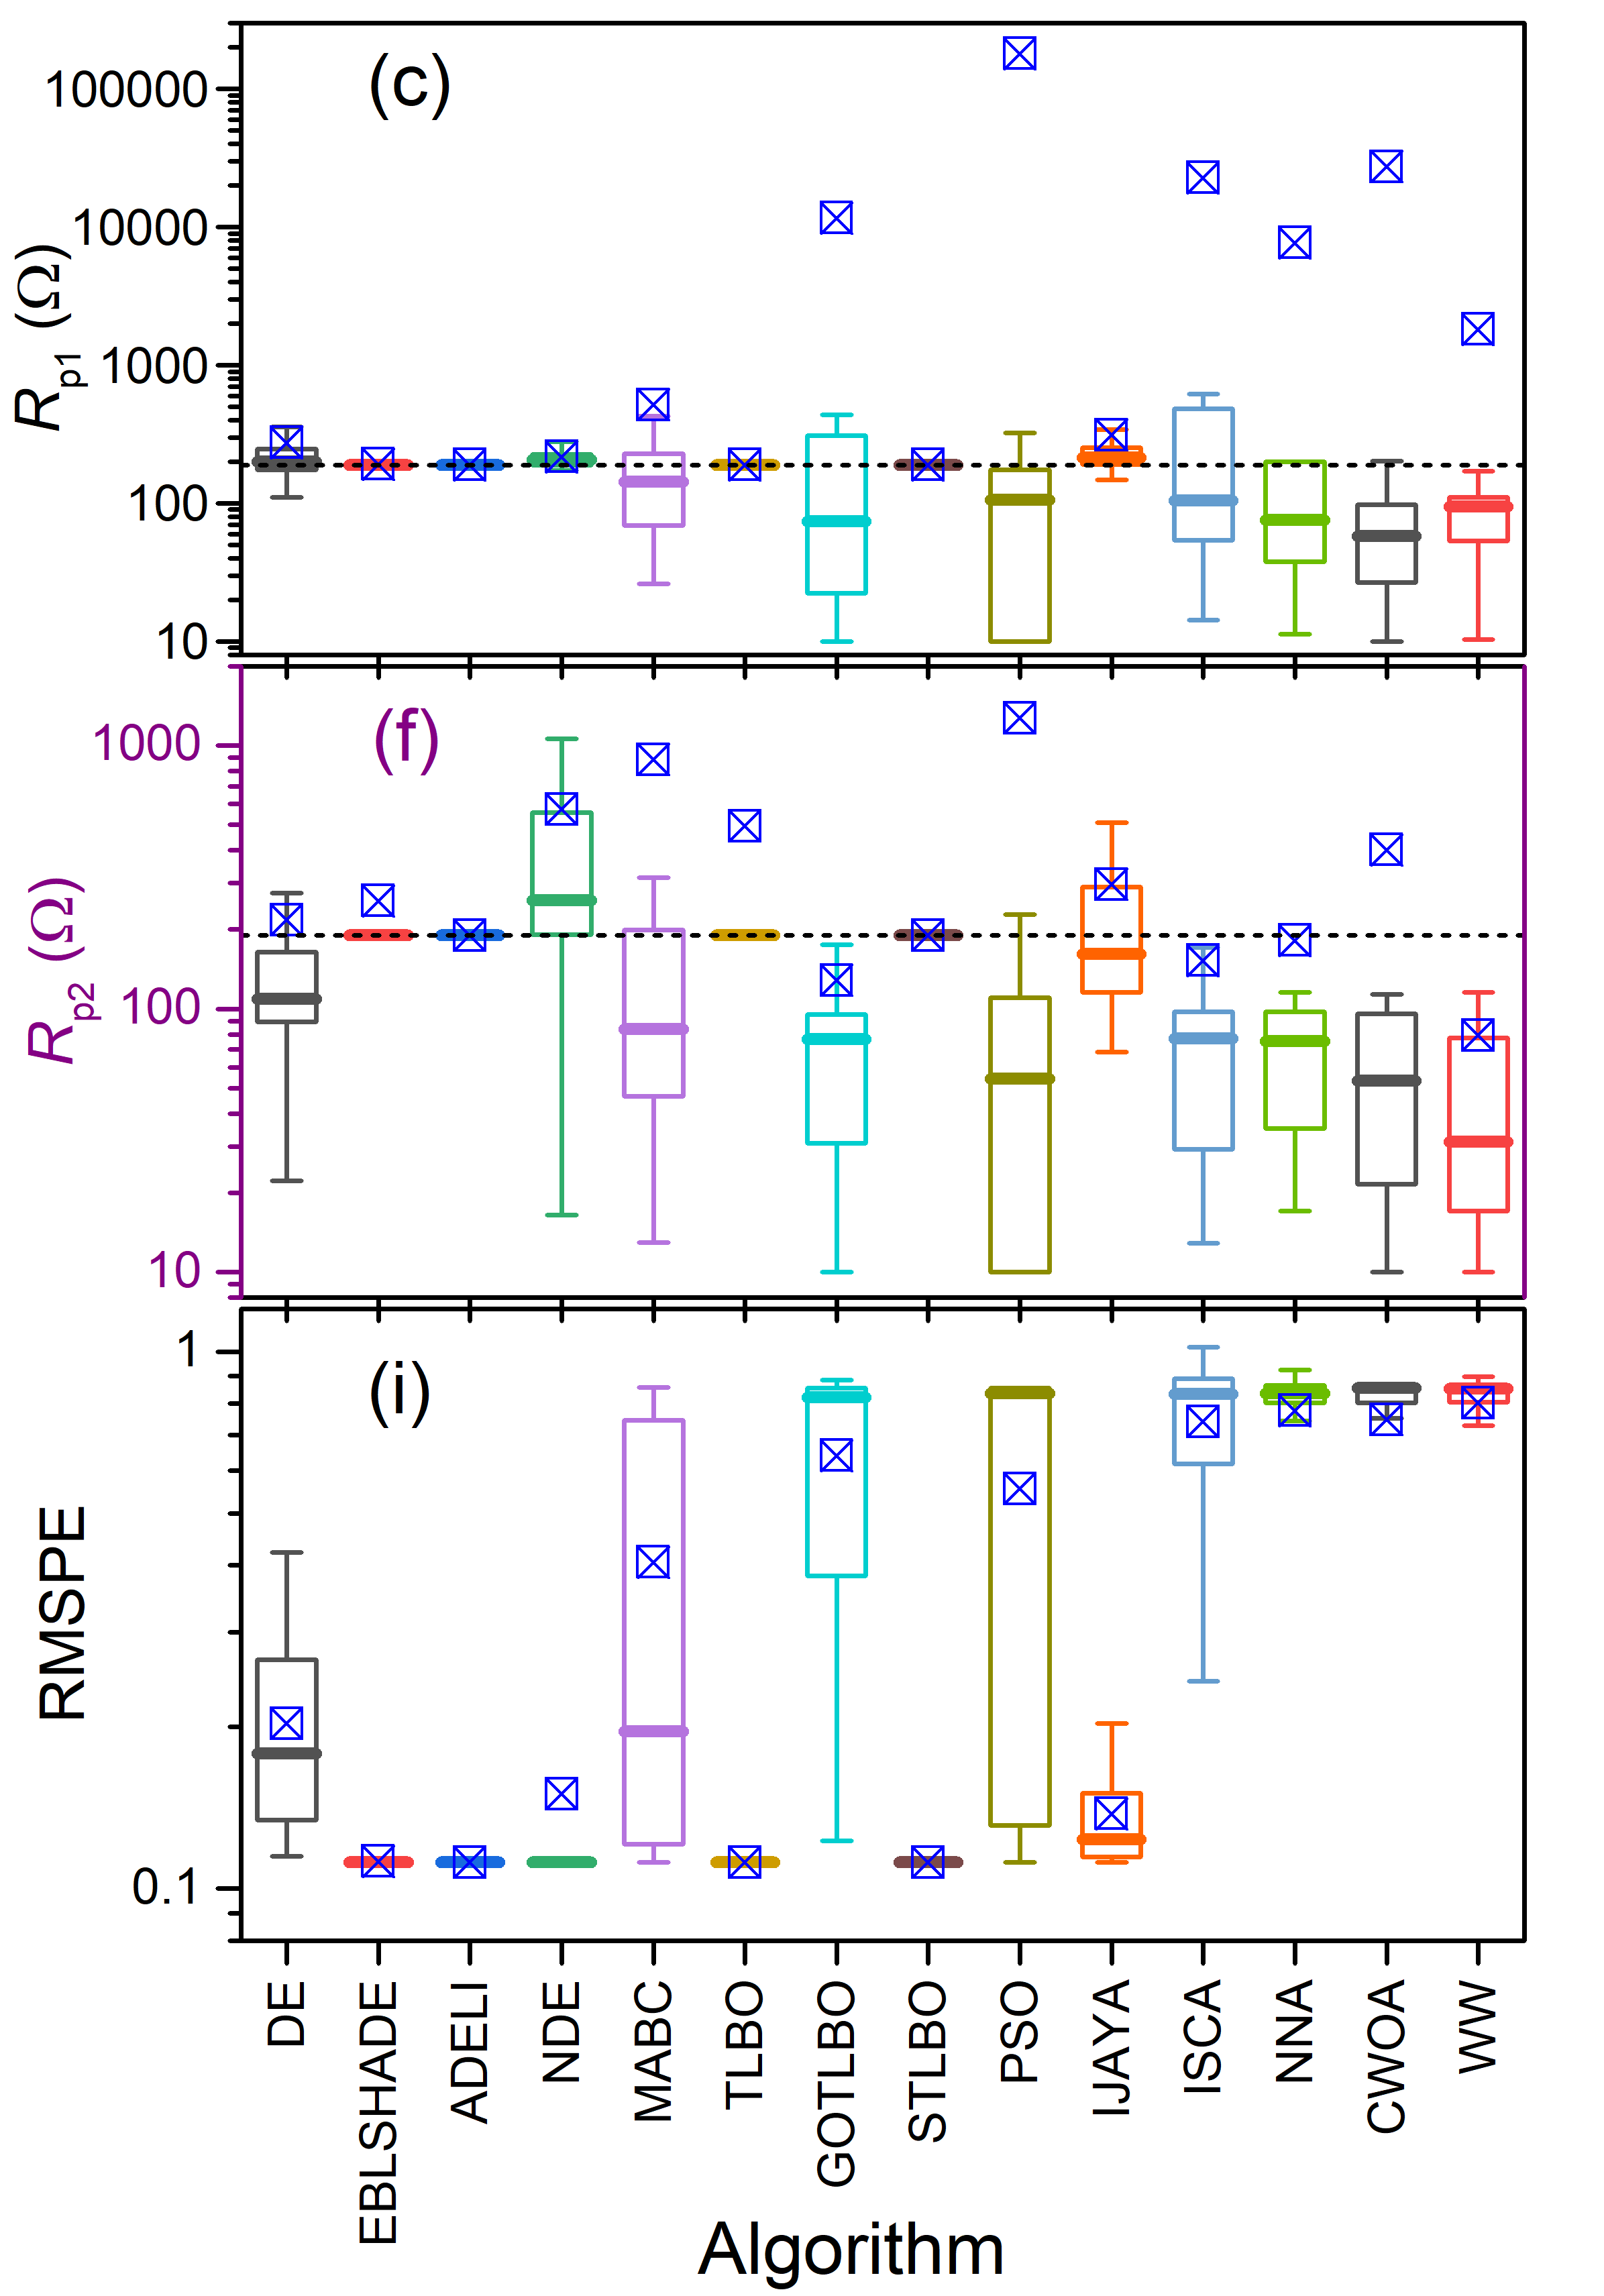
\includegraphics[width=0.4\linewidth]{Fig3c.png}
  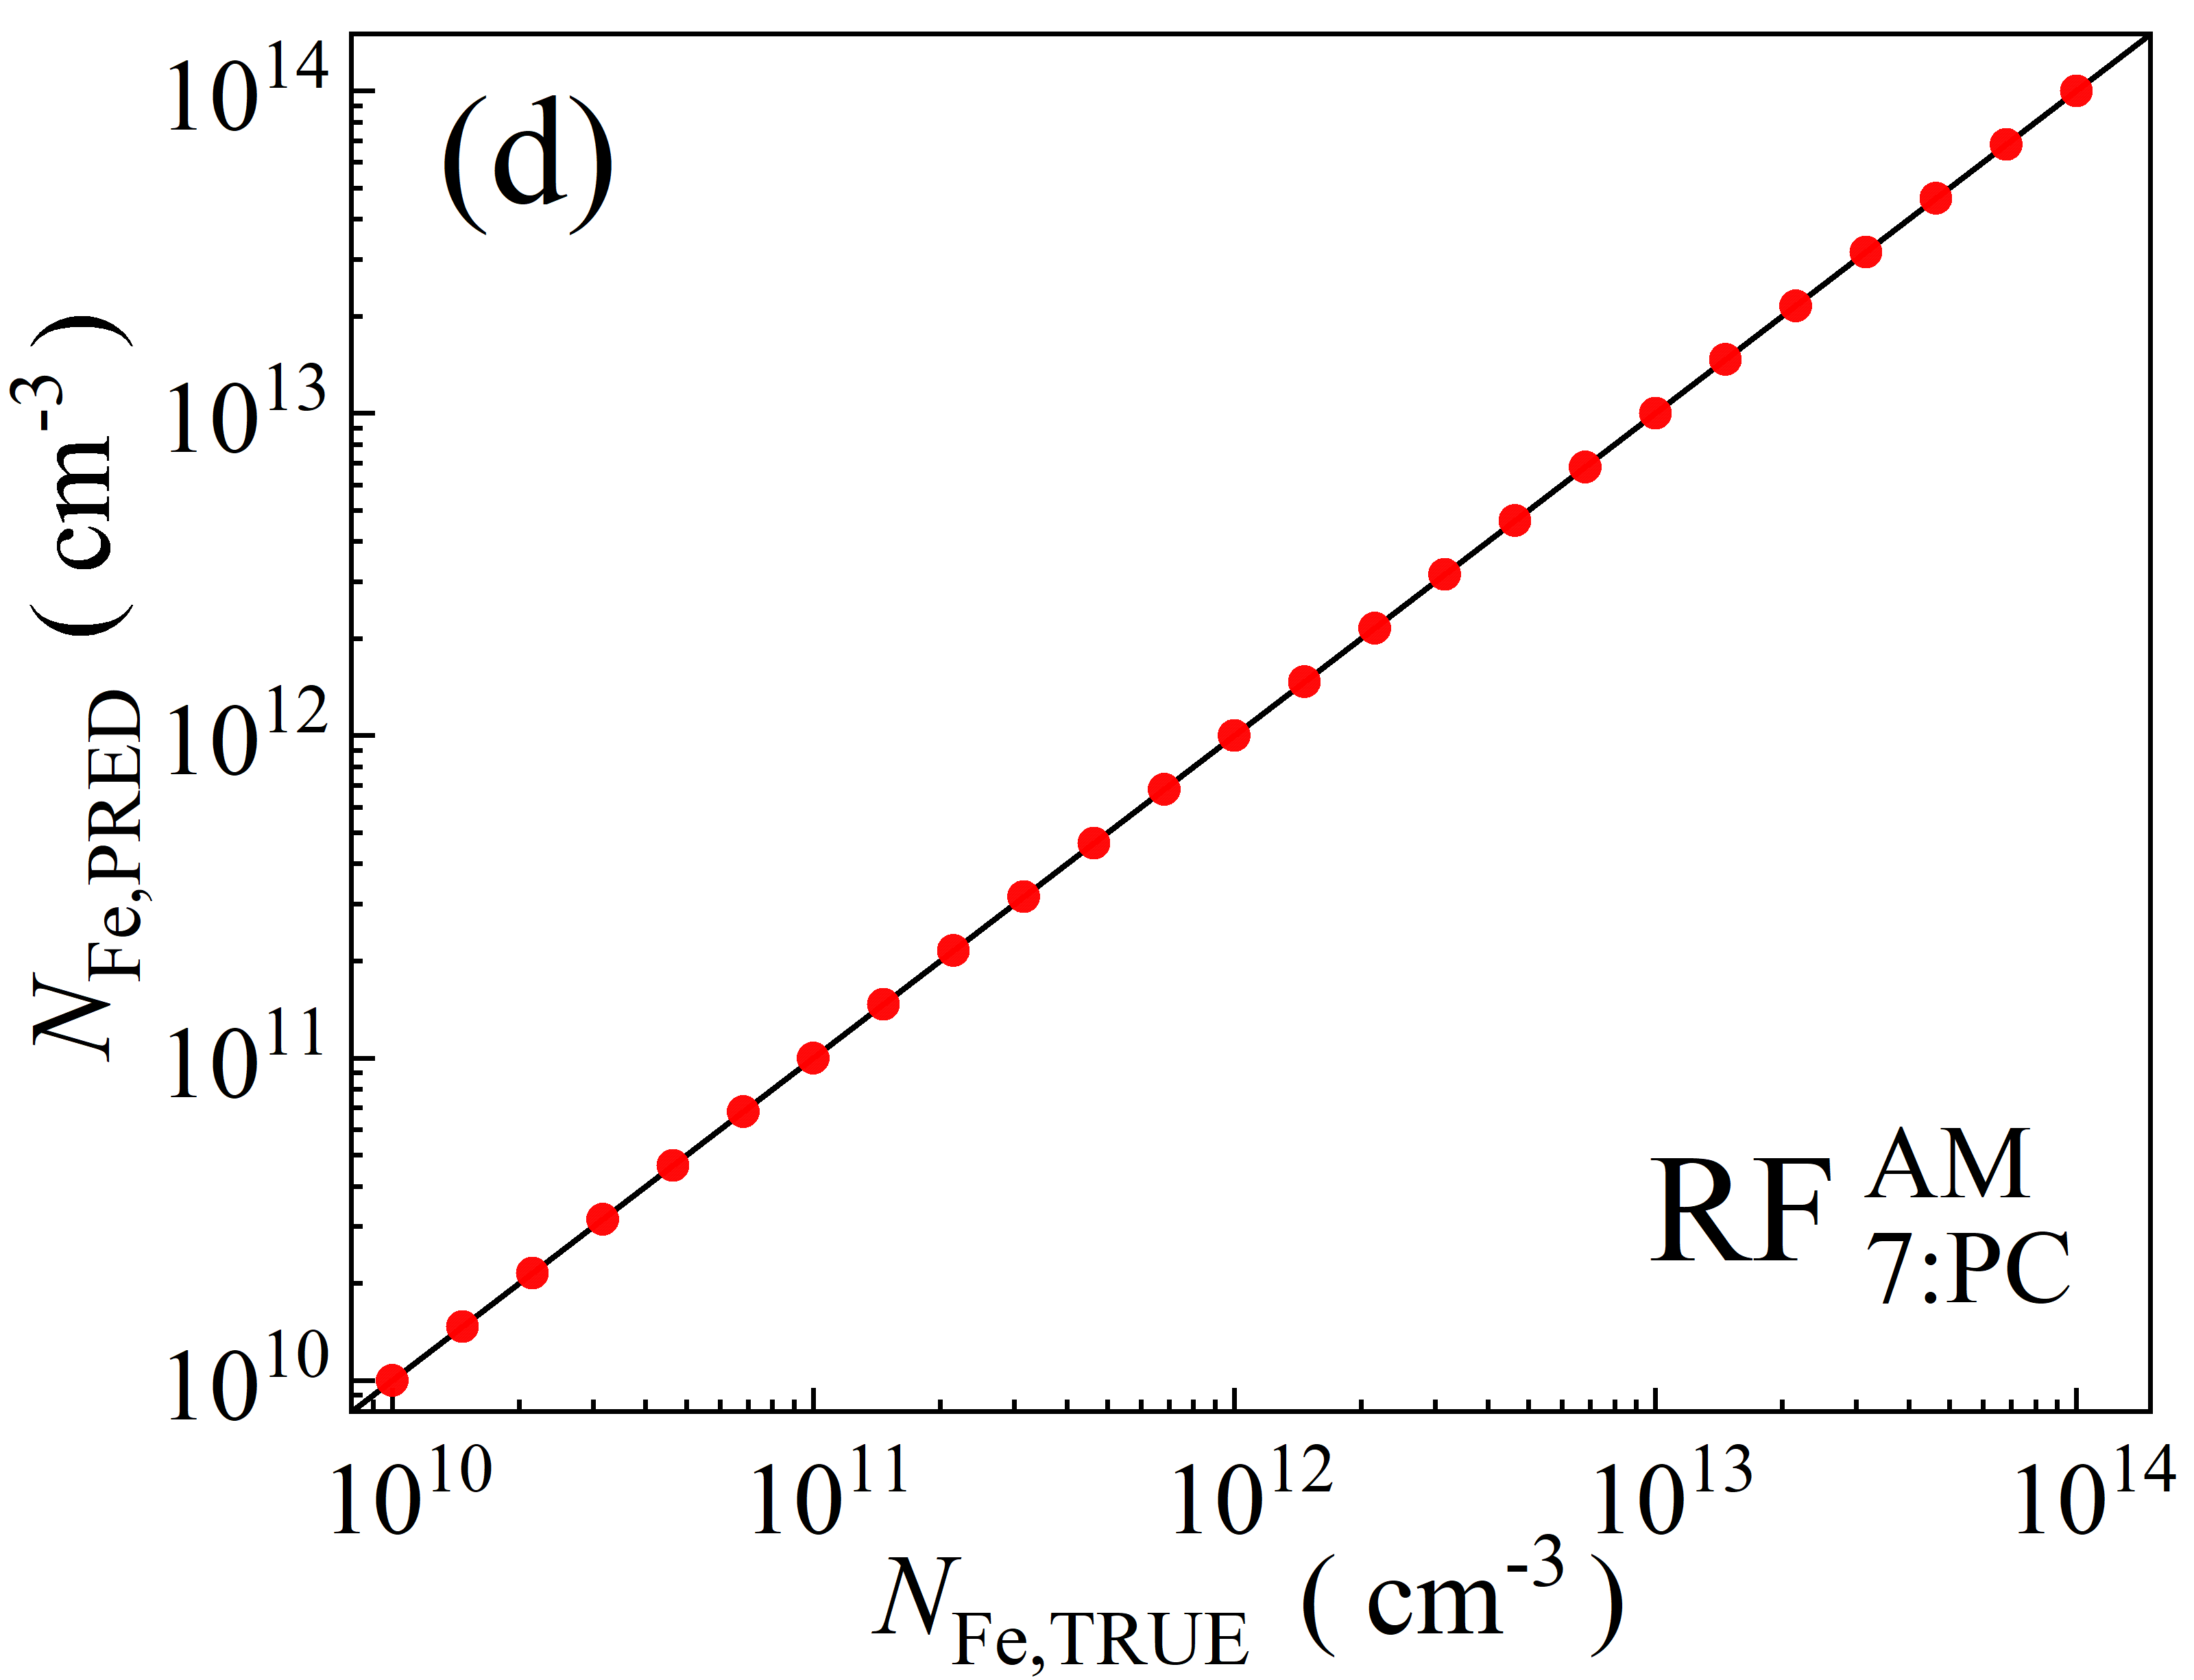
\includegraphics[width=0.4\linewidth]{Fig3d.png}
  \caption{The relationships between the concentration of FeB pairs following intense illuminations of varying intensities and the illumination duration. 
  Light source: Orion (a), Osram (b), GE (c).
  Panel d highlights variations in the dissociation of pairs induced by different light sources. 
  The marks are the experimental results, the lines are the fitted curves using Eq.~(\ref{eqIsc}).
  $T=340$~K.}
  \label{fig3}
\end{figure}

\begin{table}
 \caption{The value of maximum concentrations of iron atoms after illumination and
characteristic dissociation time obtained by approximating experimental dependencies by Eq.~(\ref{eqIsc}).
Coefficient of determination is listed as well.}
 \label{tb1}
  \begin{tabular}[htbp]{@{}ccccc@{}}
    \hline
    $W_\mathrm{ill}$~[mW] & Light source & $\tau_\mathrm{dis}$ [s] & $N_\mathrm{Fe,fit}$ [$10^{12}$~cm$^2$] & $R^2$ \\
    \hline
    750  & Orion  & $2.2\pm0.2$ & $8.6\pm0.1$ & 0.993 \\
    700  & Orion  & $2.4\pm0.2$ & $8.5\pm0.1$ & 0.995 \\
         & Osram  & $2.4\pm0.2$ & $8.6\pm0.1$ & 0.992 \\
    600  & Orion  & $3.7\pm0.2$ & $8.65\pm0.06$ & 0.998 \\
         & Osram  & $3.0\pm0.2$ & $8.69\pm0.08$ & 0.995 \\
    500  & Orion  & $5.5\pm0.2$ & $8.65\pm0.04$ & 0.999 \\
         & Osram  & $4.5\pm0.1$ & $8.7\pm0.1$ & 0.998 \\
    400  & Orion  & $8.8\pm0.3$ & $8.74\pm0.06$ & 0.998 \\
         & Osram  & $6.1\pm0.2$ & $8.63\pm0.08$ & 0.997 \\
         & GE  & $3.6\pm0.3$ & $8.7\pm0.1$ & 0.996 \\
    300  & Orion  & $15.7\pm0.6$ & $8.6\pm0.1$ & 0.998 \\
         & Osram  & $12.4\pm0.1$ & $8.69\pm0.02$ & 0.999 \\
         & GE  & $6.5\pm0.2$ & $8.69\pm0.05$ & 0.998 \\
    200  & Orion  & $42\pm3$ & $8.6\pm0.3$ & 0.998 \\
         & Osram  & $20.0\pm0.7$ & $8.53\pm0.09$ & 0.999 \\
         & GE  & $15.1\pm0.5$ & $8.7\pm0.1$ & 0.999 \\
    \hline
  \end{tabular}
\end{table}

\subsection{Second Subsection}



\section{Conclusion}

% Experimental section

\section{Experimental Section}
\threesubsection{First part of experimental section}\\
\threesubsection{Second part of experimental section}\\



\medskip
\textbf{Supporting Information} \par %Please delete the Suppporting Information statement if it is not applicable. Please supply Supporting Information in another file. Supporting information should not be provided in .tex format
Supporting Information is available from the Wiley Online Library or from the author.



% Acknowledgements
\medskip
\textbf{Acknowledgements} \par %delete if not applicable))
The authors are grateful for the help with calculating the coefficient of reflection by solar cells to Prof. Vitaliy Kostylyov.

\medskip
\textbf{Conflict of Interest}
The authors declare no conflict of interest.

% References
\medskip

% Use the following code if you wish to generate your bibliography with BibTeX;
% replace the string "MSP-template" below with the name(s) of
% the BibTeX data base(s) you want to use.
% The resulting bibliography-output (the content of the .bbl file)
% must be pasted back into this file before submission.
% Please also include your BibTeX data base file(s) in your submission
% so that we can re-run BibTeX if necessary.
%

\bibliographystyle{MSP}
\bibliography{olikh}




% Figures/tables and captions
% Permission statements are required for all figures reproduced or adapted from previously published articles/sources. Please also ensure that all necessary permissions to reproduce images have been received
% Please remove these statements for original figures


\begin{figure}
  
\includegraphics[width=\linewidth]{placeholder-image.png}
  \caption{Figure 1 caption goes here. Reproduced with permission.\textsuperscript{[Ref.]} Copyright Year, Publisher. }
  \label{fig:boat1}
\end{figure}

\begin{figure}
  
\includegraphics[width=\linewidth]{placeholder-image.png}
  \caption{Figure 2 caption goes here. Reproduced with permission.\textsuperscript{[Ref.]} Copyright Year, Publisher.}
  \label{fig:boat1}
\end{figure}

\begin{figure}
  
\includegraphics[width=\linewidth]{placeholder-image.png}
  \caption{Figure 3 caption goes here. Reproduced with permission.\textsuperscript{[Ref.]} Copyright Year, Publisher.}
  \label{fig:boat1}
\end{figure}

\begin{table}
 \caption{Table 1 caption}
  \begin{tabular}[htbp]{@{}lll@{}}
    \hline
    Description 1 & Description 2 & Description 3 \\
    \hline
    Row 1, Col 1  & Row 1, Col 2  & Row 1, Col 3  \\
    Row 2, Col 1  & Row 2, Col 2  & Row 2, Col 3  \\
    \hline
  \end{tabular}
\end{table}


% Please provide Biographies and photos for Essays, Feature Articles, Progress Reports, Reviews, and Perspectives for those authors who should be highlighted
% These should be at most 100 words long
% For other article types this section can be removed
% Photographs should be 40mm broad and 50 mm high

\begin{figure}
  
\includegraphics{bio-placeholder.jpg}
  \caption*{Biography}
\end{figure}

\begin{figure}
  
\includegraphics{bio-placeholder.jpg}
  \caption*{Biography}
\end{figure}

\begin{figure}
  
\includegraphics{bio-placeholder.jpg}
  \caption*{Biography}
\end{figure}

\begin{figure}
  
\includegraphics{bio-placeholder.jpg}
  \caption*{Biography}
\end{figure}


% Table of contents entry should be 50 - 60 words long
% Image should be 55 mm broad and 50 mm high or 110 mm broad and 20 mm high


\begin{figure}
\textbf{Table of Contents}\\
\medskip
  
\includegraphics{toc-image.png}
  \medskip
  \caption*{ToC Entry}
\end{figure}


\end{document}
